\chapter{Ricerca framework adatto}
\label{sec:ricerca_framework}

Una volta esaminata l'implementazione attuale e identificati i suoi principali
problemi nel capitolo precedente, è stato deciso di utilizzare un approccio DRY.
L'acronimo DRY, Don't Repeat Yourself, si riferisce al principio in Computer
Science in cui "Ogni conoscenza deve avere una rappresentazione unica, univoca e
autorevole all’interno di un sistema" descritto in \texttt{The Pragmatic
Programmer}\cite{thomas2019pragmatic}. In questo caso ne viene esteso il
significato per riferirsi all'utilizzo di framework esterni testati e che hanno
dimostrato di funzionare.

\section{Prerequisiti}
\label{sec:prerequisiti}

Viene fatta ora un'analisi esaustiva dei prerequisiti da considerare e valutare durante
il processo di ricerca \ref{sec:opzioni_possibili} e scelta \ref{sec:scelta_finale}
del framework che verrà usato per sostituire l'attuale implementazione. Si
individuano i prerequisiti fondamentali riportati di seguito.

\subsection{Utilizzo efficiente delle risorse}
\label{sub:resource_usage}

Primo prerequisito fondamentale è la possibilità di sfruttare completamente le risorse
a disposizione. Questo significa che bisognerà inizialmente favorire la
scalabilità verticale del sistema, in questo modo è possibile partire da un sistema
più semplice che verrà esteso in seguito. Scalare verticalmente comporta creare
una macchina unica più potente e risparmiare nel complesso risorse, in quanto l'overhead
del sistema operativo è presente soltanto una volta e un core può effettivamente
eseguire più task alla volta sfruttando il multithreading.

\subsection{Definizione dipendenze tramite DAG}
\label{sub:deps_definition}

Come visto nella sezione \ref{sub:robots}, vengono definite delle dipendenze tra
fasi. Uno dei prerequisiti fondamentali è la possibilità di definire in modo
esplicito grafi di dipendenze, non dovendo quindi pensare per ogni fase quali devono
essere quelle che la precedono o la seguono. Sarebbe ideale un'implementazione
analoga a quella riportata nel codice \ref{lst:dag-example} e renderizzata in
figura \ref{fig:dag-example}.

\begin{figure}[htbp]
  \centering
  \begin{minipage}{0.45\textwidth}
    \centering
    \lstinputlisting[language=Python, caption=Esempio di definizione di DAG in Airflow,
    label=lst:dag-example ]{listings/dag-example.py}
  \end{minipage}
  \hfill
  \begin{minipage}{0.45\textwidth}
    \centering
    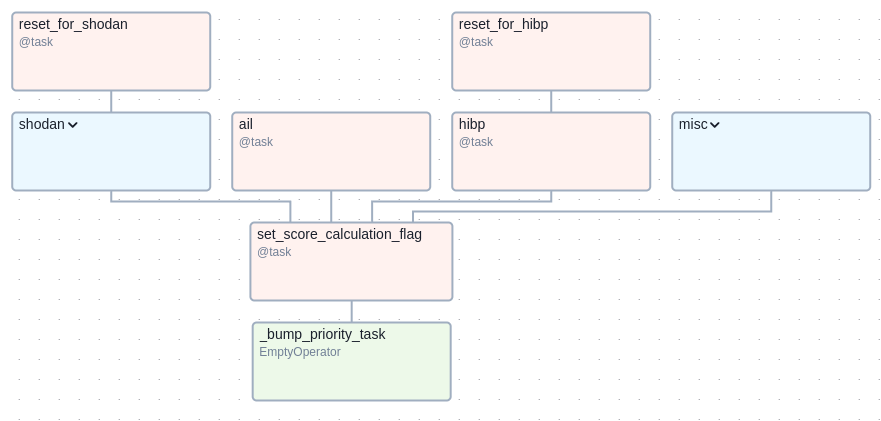
\includegraphics[width=\textwidth]{images/dag-example.png}
    \caption{Esempio di renderizzazione del DAG}
    \label{fig:dag-example}
  \end{minipage}
\end{figure}

\subsection{Compatibilità con Python}
\label{sub:python_compatibility}

compatibile nativamente con python e programmatico

\subsection{Open source, Supporto e Manutenzione}
\label{sub:open_source}

\lipsum[1]

\subsection{Facilmente scalabile}
\label{sub:scalable}

facilmente scalabile su più macchine virtuali

\subsection{Monitorabilità}
\label{sub:monitorable}

\lipsum[1]

\section{Opzioni possibili}
\label{sec:opzioni_possibili}

Durante l'attività di ricerca sono stati individuate più soluzioni e framework
che rispettavano alcuni o tutti i requisiti definiti nella sezione precedente. Di
seguito sono riportati i candidati più adeguati che sono stati valutati per la scelta
finale:
\begin{itemize}
  \item \textbf{multithreading nativo di Python:} (scartato, fai da te) \lipsum[1]

  \item \textbf{Celery\footnote{\url{https://github.com/celery/celery}}:}
    \lipsum[1]

  \item \textbf{Luigi\footnote{\url{https://github.com/spotify/luigi}}:} \lipsum[1]

  \item \textbf{Apache Airflow\cite{airflow}:} \lipsum[1]
\end{itemize}

\section{Scelta finale}
\label{sec:scelta_finale}

\lipsum[1]